DEAP is used in Darwin framework by utilizing its loose coupling design. Each of the DEAP components is configured
separately. This way the processes of Darwin framework that are dependant on DEAP can be split into multiple functions so loose coupling can
be achieved.
\paragraph{}
The \textit{Configuration} class as seen in figure \ref{lst:config} consists of the \textit{pset} and \textit{toolbox} components
from the DEAP framework. In order to set the needed information for the genetic programming an abstraction layer is added to the DEAP framework.
Because the purpose of Darwin is known - solve symbolic regression problems, there are many pre-set parameters used in the configuration, hence there are 
fewer parameters to be specified for Darwin. This level of abstraction simplifies the use of the
framework by lowering the amount of parameters needed. \textit{Configuration} provides a \textit{configure()} method
that organizes the Darwin variables and sets up the DEAP framework underneath. This \textit{configure()} method do four things as seen in \ref{fig:classdi}:

\begin{enumerate}
  \item \textit{setPrimitiveFunctions()} extracts the primitive functions from the user defined class that extends \textit{PrimitiveConfig} . It takes an instance
of each of the methods and maps them to the DEAP framework.
  \item \textit{setTerminals()} gathers a list of all defined terminals and instantiates them in the DEAP framework.
  \item \textit{configureToolbox()} is a more complex method where DEAP's \textit{toolbox} is configured:
  \begin{enumerate}
	\item Creates an individual by specifying the type of structure it is going to use (PrimitiveTree in the case). 
	\item Checks if the individual is aiming for minimum or maximum fitness function; this sets the individual to either look for lowest or 0 fitness value or the maximum among individuals.
	\item Defines the initial size of the individuals, the size of the population and generation based on the user parameters.
	\item Maps all the mutation and crossover methods to pre-defined DEAP algorithms which are good for the purpose of the genetic program.
	\item Since DEAP uses decorators to modify the generated individuals, decorators need to be defined to limit the size of an individual.
  \end{enumerate}
  \item \textit{configureArgumetns()} takes the test arguments given by the user and based on their names maps them to DEAP so the individuals can take arguments.
\end{enumerate}

\begin{landscape}
\begin{figure}[htp]
\centering
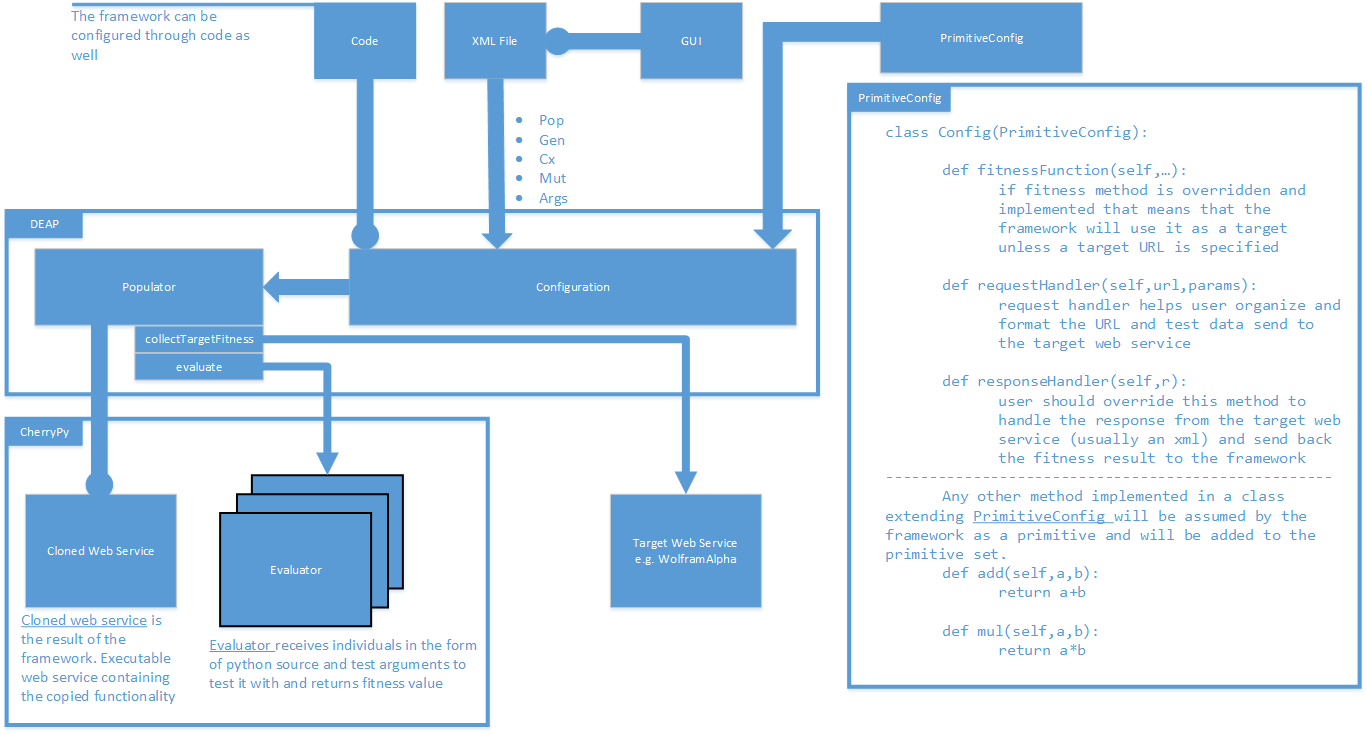
\includegraphics[scale=0.7]{Figures/Class.png}
\caption{Lower level component diagram showing the functionality and usage of each class/component (this is a copy for easier readability}
\label{fig:classdi}
\end{figure}
\end{landscape}

\begin{landscape}
\begin{lstlisting}[language=Python,caption={The core method in Configuration class that configures the DEAP framework},label={lst:config}]

def configureToolbox(self):
    if not self.isMax   : creator.create("FitnessMin", base.Fitness, weights=(-1.0,))
    else                : creator.create("FitnessMax", base.Fitness, weights=(-1.0,))

    creator.create("Individual", gp.PrimitiveTree, fitness=creator.FitnessMin, pset=self.pset)
    self.toolbox.register("expr", gp.genRamped, pset= self.pset, min_=self.depthInitialMin, max_=self.depthInitialMax)
    self.toolbox.register("individual", tools.initIterate, creator.Individual,  self.toolbox.expr)
    self.toolbox.register("population", tools.initRepeat, list,  self.toolbox.individual)
    self.toolbox.register("select", tools.selTournament, tournsize=3)
    self.toolbox.register("mate", gp.cxOnePoint)
    self.toolbox.register("expr_mut", gp.genFull, min_=0, max_=2)
    self.toolbox.register('mutate', gp.mutUniform, expr= self.toolbox.expr_mut)

	self.toolbox.decorate('mutate',gp.staticDepthLimit(self.maxDepthLimit))
    self.toolbox.decorate('mate',gp.staticDepthLimit(self.maxDepthLimit))
\end{lstlisting}
\end{landscape}	

